% Options for packages loaded elsewhere
\PassOptionsToPackage{unicode}{hyperref}
\PassOptionsToPackage{hyphens}{url}
\PassOptionsToPackage{dvipsnames,svgnames,x11names}{xcolor}
\PassOptionsToPackage{space}{xeCJK}
\documentclass[
  10pt,
]{article}
\usepackage{xcolor}
\usepackage[margin=0.70in]{geometry}
\usepackage{amsmath,amssymb}
\setcounter{secnumdepth}{-\maxdimen} % remove section numbering
\usepackage{iftex}
\ifPDFTeX
  \usepackage[T1]{fontenc}
  \usepackage[utf8]{inputenc}
  \usepackage{textcomp} % provide euro and other symbols
\else % if luatex or xetex
  \usepackage{unicode-math} % this also loads fontspec
  \defaultfontfeatures{Scale=MatchLowercase}
  \defaultfontfeatures[\rmfamily]{Ligatures=TeX,Scale=1}
\fi
\usepackage{lmodern}
\ifPDFTeX\else
  % xetex/luatex font selection
  \setmainfont[]{Cambria}
  \setmonofont[]{Consolas}
  \ifXeTeX
    \usepackage{xeCJK}
    \setCJKmainfont[]{Microsoft YaHei}
  \fi
  \ifLuaTeX
    \usepackage[]{luatexja-fontspec}
    \setmainjfont[]{Microsoft YaHei}
  \fi
\fi
% Use upquote if available, for straight quotes in verbatim environments
\IfFileExists{upquote.sty}{\usepackage{upquote}}{}
\IfFileExists{microtype.sty}{% use microtype if available
  \usepackage[]{microtype}
  \UseMicrotypeSet[protrusion]{basicmath} % disable protrusion for tt fonts
}{}
\makeatletter
\@ifundefined{KOMAClassName}{% if non-KOMA class
  \IfFileExists{parskip.sty}{%
    \usepackage{parskip}
  }{% else
    \setlength{\parindent}{0pt}
    \setlength{\parskip}{6pt plus 2pt minus 1pt}}
}{% if KOMA class
  \KOMAoptions{parskip=half}}
\makeatother
\usepackage{longtable,booktabs,array}
\newcounter{none} % for unnumbered tables
\usepackage{calc} % for calculating minipage widths
% Correct order of tables after \paragraph or \subparagraph
\usepackage{etoolbox}
\makeatletter
\patchcmd\longtable{\par}{\if@noskipsec\mbox{}\fi\par}{}{}
\makeatother
% Allow footnotes in longtable head/foot
\IfFileExists{footnotehyper.sty}{\usepackage{footnotehyper}}{\usepackage{footnote}}
\makesavenoteenv{longtable}
\usepackage{graphicx}
\makeatletter
\newsavebox\pandoc@box
\newcommand*\pandocbounded[1]{% scales image to fit in text height/width
  \sbox\pandoc@box{#1}%
  \Gscale@div\@tempa{\textheight}{\dimexpr\ht\pandoc@box+\dp\pandoc@box\relax}%
  \Gscale@div\@tempb{\linewidth}{\wd\pandoc@box}%
  \ifdim\@tempb\p@<\@tempa\p@\let\@tempa\@tempb\fi% select the smaller of both
  \ifdim\@tempa\p@<\p@\scalebox{\@tempa}{\usebox\pandoc@box}%
  \else\usebox{\pandoc@box}%
  \fi%
}
% Set default figure placement to htbp
\def\fps@figure{htbp}
\makeatother
\setlength{\emergencystretch}{3em} % prevent overfull lines
\providecommand{\tightlist}{%
  \setlength{\itemsep}{0pt}\setlength{\parskip}{0pt}}
\usepackage{bookmark}
\IfFileExists{xurl.sty}{\usepackage{xurl}}{} % add URL line breaks if available
\urlstyle{same}
\hypersetup{
  colorlinks=true,
  linkcolor={Maroon},
  filecolor={Maroon},
  citecolor={Blue},
  urlcolor={Blue},
  pdfcreator={LaTeX via pandoc}}

\author{}
\date{}

\setlength{\textfloatsep}{10pt plus 2pt minus 2pt}
\begin{document}

\section{Same-eye calibration of fundus degradation and
review}\label{same-eye-calibration-of-fundus-degradation-and-review}

Eye Sentinel · November 18, 2026 · \href{calibrated-defocus.zh.md}{中文}
· \href{calibrated-defocus.en.pdf}{PDF}

\textbf{Calibrated defocus reduced the loss in ranking performance under
mild simulated blur.} Across three matched training runs, AUROC on
original AIROGS development images rose from \textbf{0.9687 to 0.9713}.
With 3.2\% referral positives and 10\% review, false positives outside
review fell from \textbf{18.3 to 11.0 per 1,000 photos}. Misses changed
from \textbf{2.35 to 2.26 per 1,000}, with an interval that includes
zero. Each comparison lists the original mix first.

\subsection{Matched training}\label{matched-training}

{\def\LTcaptype{none} % do not increment counter
\begin{longtable}[]{@{}
  >{\raggedright\arraybackslash}p{(\linewidth - 2\tabcolsep) * \real{0.5000}}
  >{\raggedright\arraybackslash}p{(\linewidth - 2\tabcolsep) * \real{0.5000}}@{}}
\toprule\noalign{}
\begin{minipage}[b]{\linewidth}\raggedright
Item
\end{minipage} & \begin{minipage}[b]{\linewidth}\raggedright
Setting
\end{minipage} \\
\midrule\noalign{}
\endhead
\bottomrule\noalign{}
\endlastfoot
Disease classifier & EfficientNet-B0 with 320 × 320 pixel fundus
inputs \\
Training and model validation & 15,480 training images and 2,046
validation images \\
Comparison point & Three existing random seeds, weights at exactly 1,200
optimizer updates \\
Original mix & Augment about half of training draws, equally across
illumination, defocus and scatter \\
Calibrated defocus & Keep the same draws and replace the image operation
for the defocus cases \\
\end{longtable}
}

Original defocus combines Gaussian blur with noise or JPEG compression.
Calibrated defocus applies blur and exposure drawn from a parameter bank
fitted on 60 Real Fundus pairs. The experiment compares the full change
to the defocus recipe. The calibrated median radius is 1.7 pixels at a
512-pixel field and the median exposure multiplier is 0.99. The three
seeds drew defocus 3,292 / 3,228 / 3,306 times, respectively. Per-image
sampling, source and label counts, and degradation-family draws matched
the control in every seed.

\begin{figure}
\centering
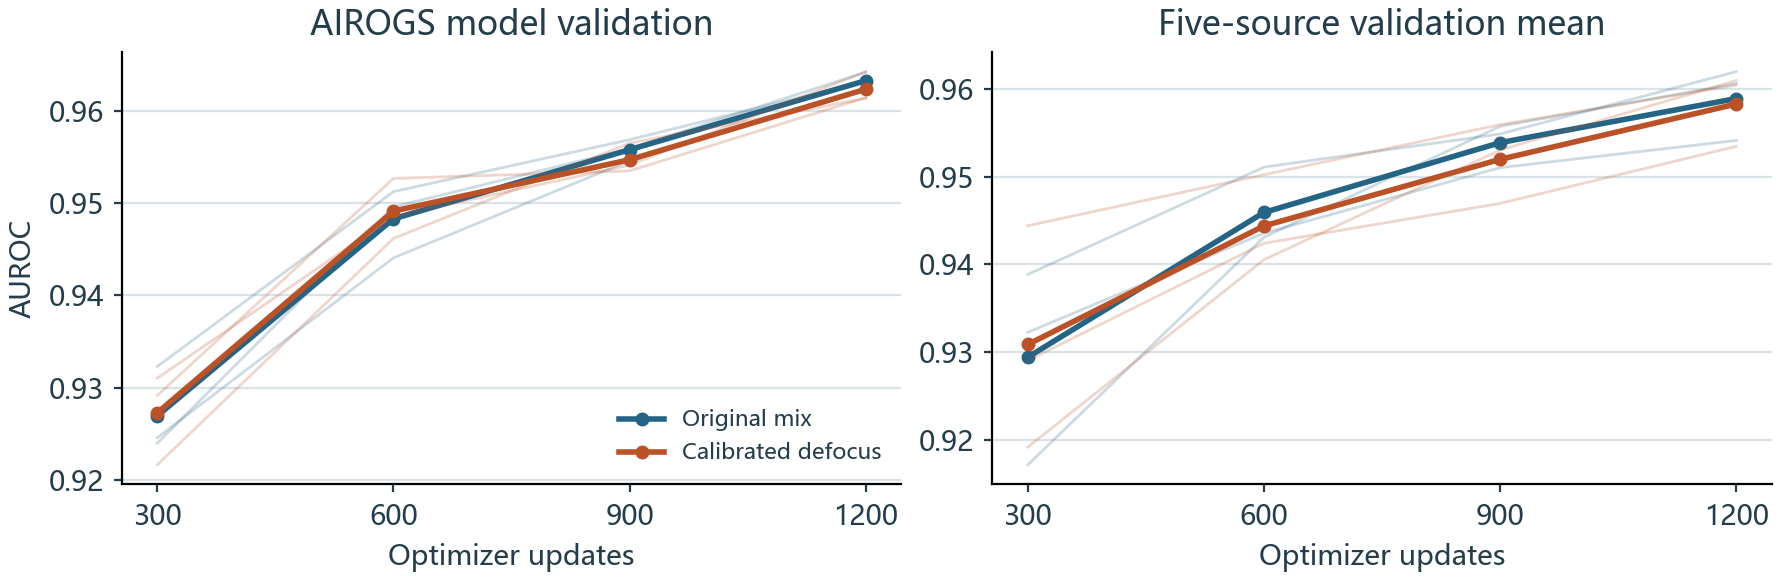
\includegraphics[width=0.98\linewidth,height=\textheight,keepaspectratio,alt={Each thin trace represents a seed. Solid lines show the three-seed means. The right panel averages validation AUROC equally across AIROGS, ODIR, Kaggle, LAG and KEH.}]{calibrated-validation.en.png}
\caption{Each thin trace represents a seed. Solid lines show the
three-seed means. The right panel averages validation AUROC equally
across AIROGS, ODIR, Kaggle, LAG and KEH.}
\end{figure}

\textbf{AUROC} is the probability that a randomly chosen positive
receives a higher score than a randomly chosen negative, with ties
counted as half. Validation was run every 300 updates. The pilot
compares the prespecified update-1,200 checkpoints on development data.
The reserved independent tests remain sealed.
\href{../../../data/prepared/expanded_20261113/README.en.md}{Frozen data
release} ·
\href{../../../configs/calibrated_defocus_20261118/profile.json}{Calibration
profile} ·
\href{../../../tools/run_calibrated_defocus_20261118.py}{Training code}
·
\href{../../../tools/evaluate_calibrated_defocus_20261118.py}{Evaluation
code}

\newpage

\subsection{Originals, simulated blur and real low-quality
images}\label{originals-simulated-blur-and-real-low-quality-images}

{\def\LTcaptype{none} % do not increment counter
\begin{longtable}[]{@{}
  >{\raggedright\arraybackslash}p{(\linewidth - 6\tabcolsep) * \real{0.2000}}
  >{\raggedleft\arraybackslash}p{(\linewidth - 6\tabcolsep) * \real{0.2667}}
  >{\raggedleft\arraybackslash}p{(\linewidth - 6\tabcolsep) * \real{0.2667}}
  >{\raggedleft\arraybackslash}p{(\linewidth - 6\tabcolsep) * \real{0.2667}}@{}}
\toprule\noalign{}
\begin{minipage}[b]{\linewidth}\raggedright
Development condition
\end{minipage} & \begin{minipage}[b]{\linewidth}\raggedleft
Images
\end{minipage} & \begin{minipage}[b]{\linewidth}\raggedleft
Original mix AUROC
\end{minipage} & \begin{minipage}[b]{\linewidth}\raggedleft
Calibrated defocus AUROC
\end{minipage} \\
\midrule\noalign{}
\endhead
\bottomrule\noalign{}
\endlastfoot
All development originals & 2,053 & 0.9716 & 0.9731 \\
AIROGS development originals & 773 & 0.9687 & 0.9713 \\
Originals in blur subset & 384 & 0.9755 & 0.9777 \\
Mild blur & 384 & 0.9496 & 0.9669 \\
Strong blur & 384 & 0.9000 & 0.9115 \\
\end{longtable}
}

\begin{figure}
\centering
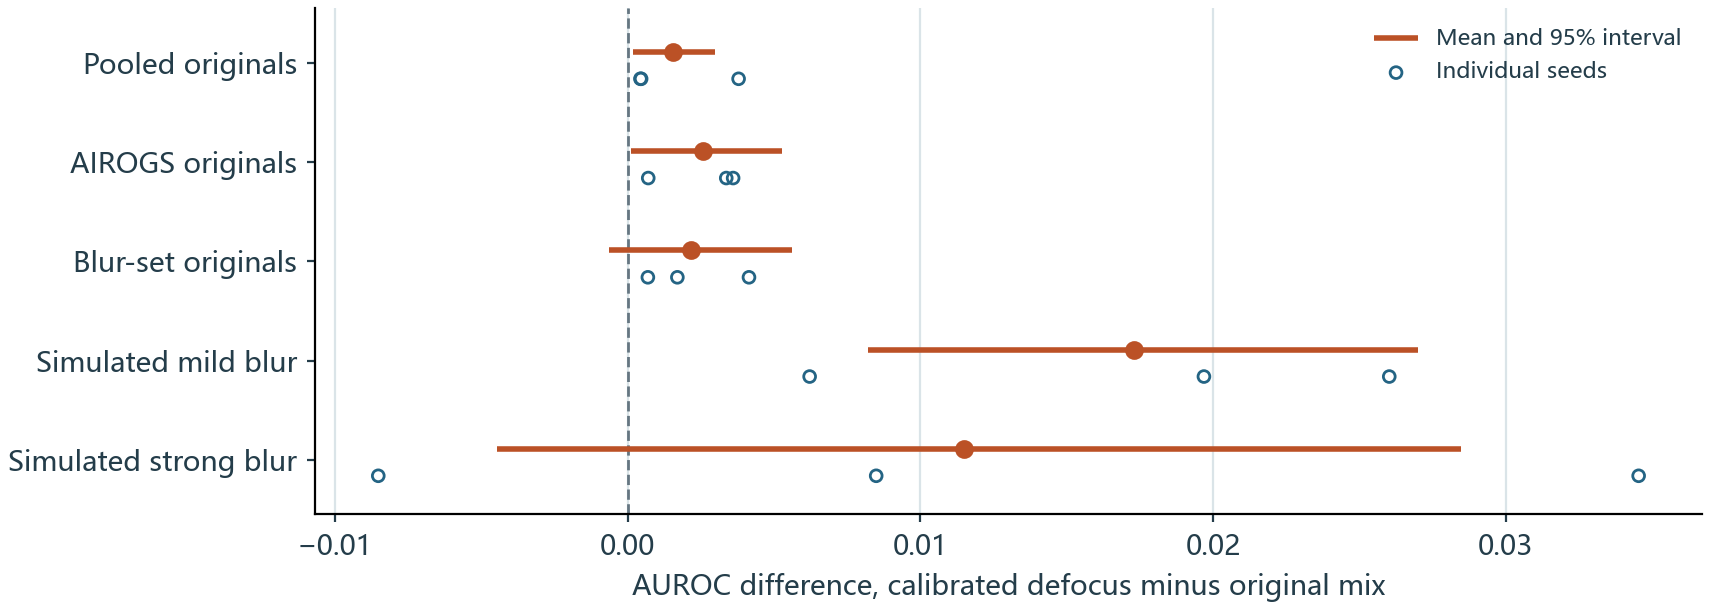
\includegraphics[width=0.98\linewidth,height=\textheight,keepaspectratio,alt={Open circles show AUROC differences by seed. Filled circles show means and bars show 95\% intervals. Values to the right favor calibrated defocus.}]{calibrated-development-auroc.en.png}
\caption{Open circles show AUROC differences by seed. Filled circles
show means and bars show 95\% intervals. Values to the right favor
calibrated defocus.}
\end{figure}

We kept the same 384 images and applied both blur levels to each. At a
512-pixel field, Gaussian blur radii were 2 and 5 pixels. After
accounting for the difference on those same originals, the
\textbf{difference in AUROC change} was \textbf{+0.0151} {[}+0.0070,
+0.0236{]} under mild blur and \textbf{+0.0093} {[}-0.0060, +0.0251{]}
under strong blur. A positive value means the calibrated arm lost less
AUROC. Intervals use 2,000 paired linked-group resamples with the three
seeds fixed. A linked group keeps photographs of the same known patient
or related images together.

AIROGS positives met the reference criteria for glaucoma referral.
Pooled originals and the blur subset also include other sources with
their own label definitions. They measure comparative model behavior
across this group of datasets.

{\def\LTcaptype{none} % do not increment counter
\begin{longtable}[]{@{}
  >{\raggedright\arraybackslash}p{(\linewidth - 6\tabcolsep) * \real{0.2143}}
  >{\raggedleft\arraybackslash}p{(\linewidth - 6\tabcolsep) * \real{0.2857}}
  >{\raggedleft\arraybackslash}p{(\linewidth - 6\tabcolsep) * \real{0.2857}}
  >{\raggedright\arraybackslash}p{(\linewidth - 6\tabcolsep) * \real{0.2143}}@{}}
\toprule\noalign{}
\begin{minipage}[b]{\linewidth}\raggedright
Quality group in real originals
\end{minipage} & \begin{minipage}[b]{\linewidth}\raggedleft
Positive
\end{minipage} & \begin{minipage}[b]{\linewidth}\raggedleft
Negative
\end{minipage} & \begin{minipage}[b]{\linewidth}\raggedright
Positive calls at a disease score \textgreater{} 0.5 by seed
\end{minipage} \\
\midrule\noalign{}
\endhead
\bottomrule\noalign{}
\endlastfoot
Human-labeled low quality & 12 & 0 & Original 12 / 12 / 11 · Calibrated
12 / 12 / 12 \\
Model quality score below 0.20 & 29 & 38 & Original 25 / 27 / 26 ·
Calibrated 24 / 27 / 28 \\
\end{longtable}
}

FIVES marks poor focus, illumination or contrast. MSHF uses a poor
overall quality grade. The low model-quality group has an EyeQ--FTHNet
score below 0.20. The human-labeled subgroup contains no negatives, so
it cannot estimate false positives there.
\href{https://www.nature.com/articles/s41597-022-01564-3}{FIVES dataset}
· \href{https://www.nature.com/articles/s41597-023-02188-x}{MSHF
dataset}

\newpage

\subsection{What the simulation
reproduces}\label{what-the-simulation-reproduces}

We fit a profile on 60 Real Fundus pairs and compared image versions on
60 other pairs. The split uses photo-pair IDs because patient IDs are
unavailable. Starting from the clearer photograph, we compared the real
poorer photo with the original mix, the author versions of CoFe and
ArcNet, and calibrated blur plus exposure.

\begin{figure}
\centering
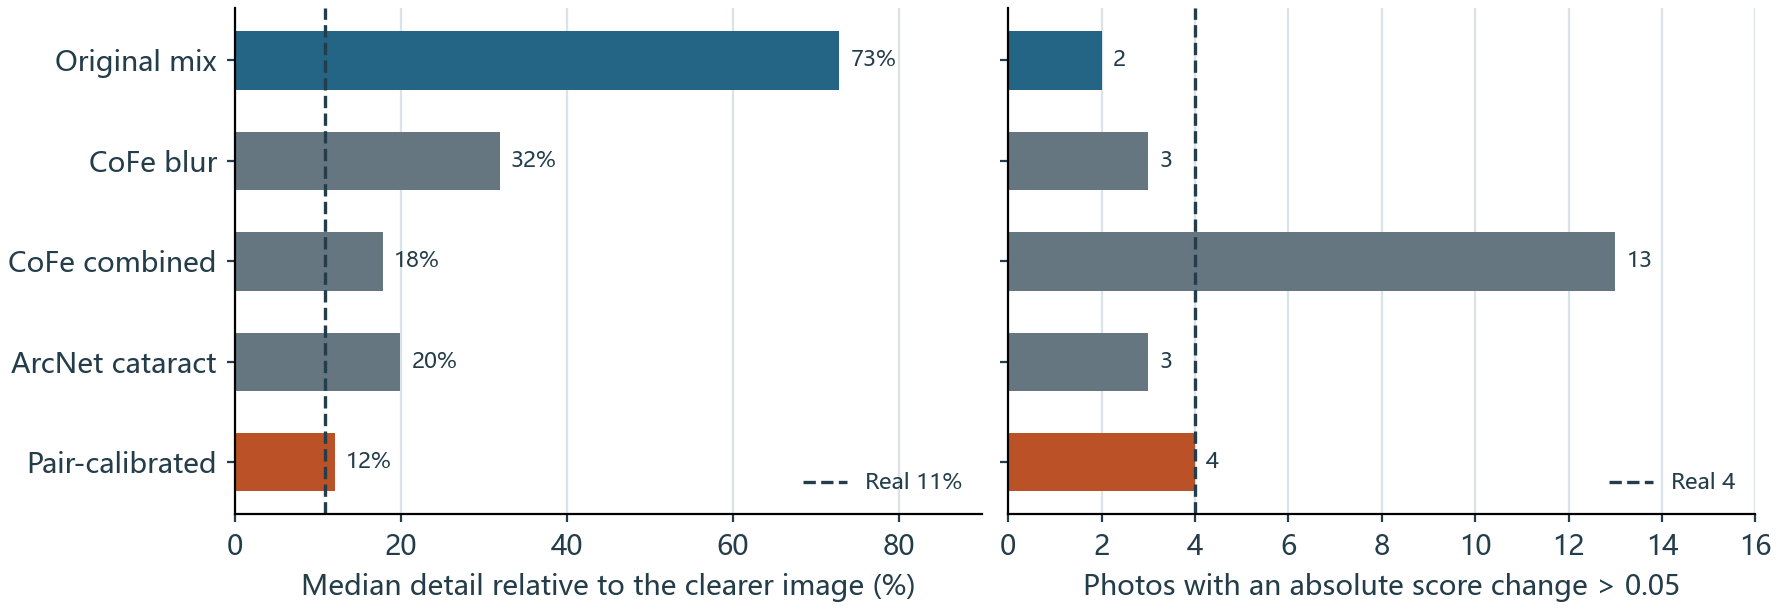
\includegraphics[width=0.98\linewidth,height=\textheight,keepaspectratio,alt={Dashed lines show the real poorer photo. The left panel uses the ratio of green-channel Laplacian variance, which responds to edges and local intensity changes. The right panel counts large disease-score shifts among 60 photos.}]{calibrated-image-benchmark.en.png}
\caption{Dashed lines show the real poorer photo. The left panel uses
the ratio of green-channel Laplacian variance, which responds to edges
and local intensity changes. The right panel counts large disease-score
shifts among 60 photos.}
\end{figure}

The median detail statistic relative to the clearer same-eye photo was
\textbf{11\%} for real poorer photos, \textbf{73\%} for the original
mix, and \textbf{12\%} for calibrated blur plus exposure. The combined
CoFe simulation and ArcNet cataract simulation retained \textbf{18\%}
and \textbf{20\%}. Their outputs were respectively darker and brighter
than the real poorer photos on the mean luminance measure. They provide
distinct acquisition stress tests.
\href{https://arxiv.org/abs/2201.00466}{Real Fundus} ·
\href{https://arxiv.org/abs/2005.05594}{CoFe-Net} ·
\href{https://arxiv.org/abs/2203.07737}{ArcNet}

Calibration improved agreement on the detail statistic. Under the same
frozen disease classifier, an absolute score change greater than 0.05
occurred in \textbf{4/60} real pairs, \textbf{2/60} using the original
mix and \textbf{4/60} using calibrated blur plus exposure. The original
mix was slightly closer across the full distribution of score changes.
These pairs have quality comparisons and lack glaucoma reference
outcomes. A Rotterdam population study inspected 100 ungradable
photographs and found incomplete optic disc capture in 98. The next
acquisition study should record whether the disc is fully in frame.
\href{https://www.aaojournal.org/article/S0161-6420\%2826\%2900846-8/fulltext}{Population
screening study} · \href{review-degradation-benchmark.json}{Image
metrics and scores}

\newpage

\subsection{At a 10\% review budget}\label{at-a-10-review-budget}

We reweighted 773 AIROGS development photos to \textbf{3.2\% referral
positives} and reviewed 100 per 1,000. Each model used the 95th
percentile of its negative validation scores as its classification
threshold. The gray zone prioritized scores close to that threshold and
lower quality. A miss is a negative call on a reference-positive photo.
A false positive is a referral call on a reference-negative photo.
Outside review refers to photos omitted from the review list.

\begin{figure}
\centering
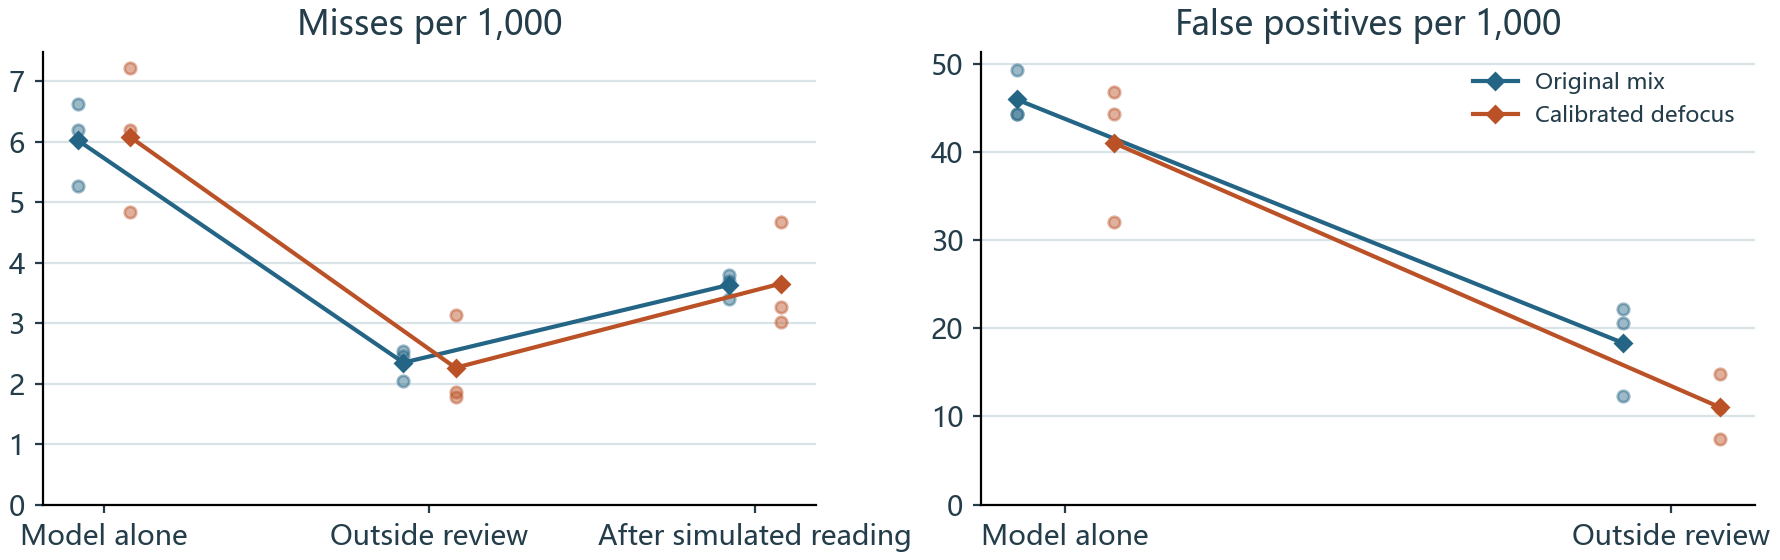
\includegraphics[width=0.92\linewidth,height=\textheight,keepaspectratio,alt={Dots show seeds and diamonds show means. The last point on the left assumes reader sensitivity of 86\% and specificity of 96.4\%. The right panel shows false positives before routing and outside review.}]{calibrated-review-routing.en.png}
\caption{Dots show seeds and diamonds show means. The last point on the
left assumes reader sensitivity of 86\% and specificity of 96.4\%. The
right panel shows false positives before routing and outside review.}
\end{figure}

Per 1,000 photos, misses outside review changed by \textbf{−0.08}, with
a 95\% interval of {[}−0.47, +0.40{]}. False positives changed by
\textbf{−7.30}, with an interval of {[}−14.27, −1.46{]}. The gray zone
routed \textbf{60.3\%} and \textbf{70.1\%} of initial model errors.
Under the reader scenario, final missed referrals were \textbf{3.63 to
3.65} per 1,000.

\begin{figure}
\centering
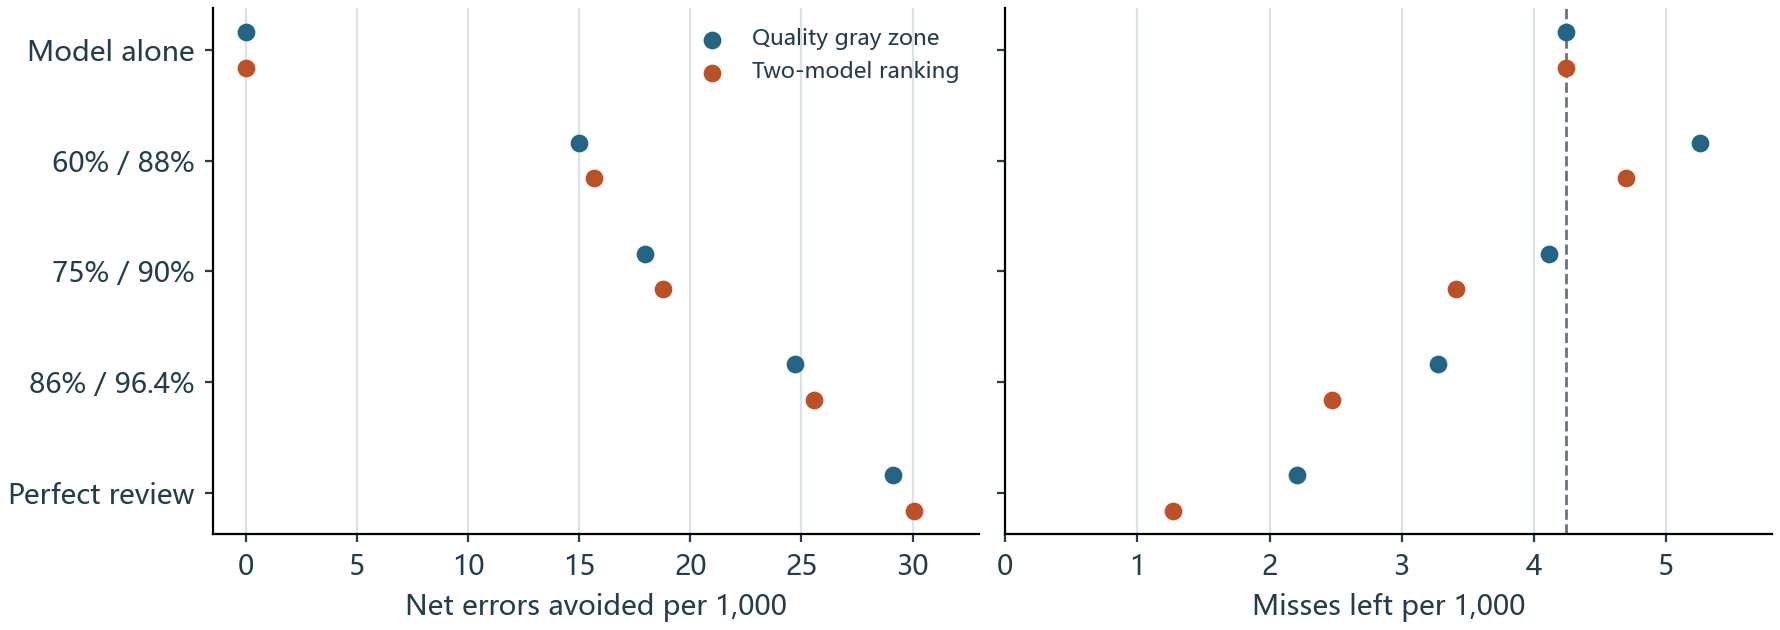
\includegraphics[width=0.92\linewidth,height=\textheight,keepaspectratio,alt={Earlier comparison at update 2,400. The paired percentages show reader sensitivity and specificity. The vertical line marks misses using the model alone. Two-model ranking uses the second model to help prioritize negative calls for review.}]{calibrated-expert-scenarios.en.png}
\caption{Earlier comparison at update 2,400. The paired percentages show
reader sensitivity and specificity. The vertical line marks misses using
the model alone. Two-model ranking uses the second model to help
prioritize negative calls for review.}
\end{figure}

The trained EyePACS readers achieved 86\% sensitivity and 96.4\%
specificity, used here as a scenario for the review list. Sensitivity is
the share of positives read correctly. Specificity is the share of
negatives read correctly. At lower sensitivity, total errors can fall
while missed referrals rise. Clinical benefit requires patient-level
evaluation with independent reference examinations and final referral
outcomes. \href{https://pubmed.ncbi.nlm.nih.gov/37113471/}{EyePACS
reader study} · \href{review-failures.en.md}{Earlier two-model analysis}
· \href{calibrated-defocus-results.json}{Results and hashes}

\end{document}
